\documentclass[letterpaper]{article}
\usepackage{amsmath}
\usepackage{amsthm}
\usepackage{systeme}
\usepackage{mdframed}
\usepackage{tikz}
\usetikzlibrary{automata,positioning}

\newtheorem{thm}{Theorem}[section]

\theoremstyle{definition}
\newtheorem{prop}[thm]{Proposition}
\newtheorem{corollary}{Corollary}[thm]
\newtheorem{lemma}[thm]{Lemma}
\newtheorem{example}[thm]{Example}
\newtheorem{definition}[thm]{Definition}

\theoremstyle{remark}
\newtheorem*{solution}{Solution}

\theoremstyle{definition}
\newtheorem{exercise}[thm]{Exercise}
\usepackage[english]{babel}
\usepackage[utf8]{inputenc}
\usepackage{graphicx}
\usepackage[colorinlistoftodos]{todonotes}

\title{Expected Value}
\author{Nathan Zhao}

\date{\today}

\begin{document}
\maketitle

\begin{abstract}
In this handout we will be discussing expected value problems common within the AMC Series.
\end{abstract}

\section{Introduction}
\begin{mdframed}
    \begin{definition}
        The expected value is the weighted average of a random variable with the values being its possible values, and the probabilities being the weights.
    \end{definition}
\end{mdframed}

So, lets portray this with simple problem: What is the expected value of a dice roll? Take a few seconds, and think about your answer. You should get $3.5$, where we get this by averaging all our possible outcomes (Numbers $1-6$). We see this is characteristic of our definition as our answer is $$\frac{1}{6} \cdot \left(\sum_{n=1}^{6} n \right)$$.

\begin{example}
Now, let us try something else. Say we have a spinner with labeled numbers. It has $\frac{1}{6}$ chance of landing on $2$, $\frac{1}{2}$ chance of landing on $3$, and $\frac{1}{3}$ chance of landing on $4$. If we spin the spinner, what is the expected value?
\end{example}

\begin{solution}
In order to solve this, we continue to use the definition of expected value. For In our problem, our calculations would look like

$$\frac{1}{6}(2) + \frac{1}{2}(3) + \frac{1}{3}(4)$$
This turns out to be $\boxed{\frac{19}{6}}$.\\
Notice that this is not actually an obtainable value on the spinner. The expected value doesn't concern what can actually happen, it represents the average value if you found the random value infinitely many times.\\
\end{solution}

\noindent
%The way we utilize our definition is by multiplying our probabilities with their associated values, and simply taking the sum. The way we did our calculation is also known as using \textbf{weighted averages}.

\subsection*{Exercises}
Now, let's try some practice. As with other future chapters, note that though these problems utilize our main topic, other different techniques are incorporated into them as well:

\begin{exercise}
    John flips a coin until he flips heads. What is the expected number of heads he will get?
\end{exercise}

\begin{exercise}
    Casey alternates flipping a coin and rolling dice, starting with the coin. She stops when she either flips tails or rolls a $6$. What is the sum of the number of tails and $1$s she will receive?
\end{exercise}

\begin{exercise}
    Brendan has a $\frac{1}{2}$ chance of hitting a tennis ball during a game, and Sally has a $\frac{1}{3}$ chance of hitting the tennis ball. What is the expected number of times the ball will be hit in a tennis game between Brendan and Sally, where Brendan serves first with $100\%$ accuracy?
\end{exercise}

\section{Linearity of Expectation}
The Linearity of Expectation purely says that $E[a+b] = E[a] + E[b]$, even if the two expected values are $\emph{dependent}$ on each other. This is very useful, as it allows us to avoid large amounts of casework and simplify complex problems.

\begin{example}
Say we flip $9$ coins and order them in a line. How many adjacent heads-heads pairs would we expect?
\end{example}

\begin{solution}
We see that we have $8$ adjacent pairs. Even though the probability for our coin-pairs depend on each other, we can still sum their expected values. So, to solve, since each adjacent pair has $\frac{1}{4}$ probability of being heads-heads, our answer is simply $8\cdot\frac{1}{4}$, or $2$. Essentially, even though our probabilities are dependent on each other (the each central coin is involved in multiple pairs), we can still simply regard them separately.\\
\end{solution}

\noindent
Apart from simplifying problems, we can use a symmetry argument along with the Linearity of Expectation to equally divide our probabilities. Let us use a problem to illustrate this principal:

\begin{example}
(Mock AIME 2 2006-2007) In his spare time, Richard shuffles a standard deck of $52$ playing cards. He then turns the cards up one by one from the top of the deck until the third ace appears. How many cards would Richard expect to flip?
\end{example}

\begin{solution}
To solve this problem, we know that there are $4$ aces in a deck, which separate the rest of the $48$ cards into $5$ groups. Understanding symmetry, we see that we expect $\frac{48}{5}$ cards on average within these groups. Since Richard stops turning cards until his third, we will go through $3$ of our card-groups and flip up $3$ additional aces. Thus, our answer is $3\cdot\frac{48}{5} + 3$ or $\frac{159}{5}$.
\end{solution}

Note that often in these problems, it is useful to split large systems into small sub-problems and easier-to-find expected values. Then, applying the Linearity of Expectation, you can essentially add your values (different for each problem of course).

\subsection*{Exercises}
Now, lets practice!

\begin{exercise}
    A group of $12$ children are doing a gift exchange, and each placing their gift in a pile. One at a time, the children randomly pick the gifts and unwrap them. After all gifts have been chosen, how many children do you expect picked their own gift?
\end{exercise}

\begin{exercise}
    (Brilliant) The digits $1$, $2$, $3$, and $4$ are randomly arranged to form two two-digit numbers, $\overline{AB}$ and $\overline{CD}$. For example, we could have $\overline{AB} = 42$ and $\overline{CD} = 13$. What is the expected value of $\overline{AB}\cdot \overline{CD}$? 
\end{exercise}

\begin{exercise}
    With $n$ people in a room, how many distinct birthdays in a $365$ day year would you expect within the room? Write your answer as an equation.
\end{exercise}

\section{Utilizing States}
States are conditions at certain point in a problem. These conditions can often be described using certain equations. Once these equations have been written, all one must do is solve the system of equations.

However, often, many people struggle with creating these equations. So, to explain, each state basically is equal to the weighted averages of the next possible states. However,
with problems that require the use of counting of a value (e.g. the number of years passed), you also have to add accordingly. Additionally, once you have a state where your counting would stop, it should equal 0.

\begin{example}
Say we have 3 switches. Every minute, a person walks by and flips a random switch (from on to off, or off to on). Initially, all the switches are off. What is the expected number of minutes until all the switches are on?
\end{example}

\begin{solution}
We solve this by creating states. Our notation for this problem will be that we use $E_{n}$ for a state where $n$ switches are active. Starting off, our state for our initial configuration $E_{0} = E_{1} + 1$. This equation results from us knowing that at $E_{0}$, we have $\frac{1}{1}$ (or $1$) chance to reach $E_{1}$. Additionally, we add $1$ in order to account for the increase in minutes. We continue to use our "coefficient as probability" idea process to create a full system of equations:

\[ \left\{ 
    \begin{array}{lcl} 
        E_{0} &= &E_{1} + 1\\
        E_{1} &= &\frac{1}{3}E_{0} + \frac{2}{3}E_{2} + 1\\
        E_{2} &= &\frac{2}{3}E_{1} + \frac{1}{3}E_{3} + 1\\
        E_{3} &= &0
\end{array}
\right.\]

Note that $E_{3} = 0$ because once all our switches are on, we don't need to count anymore. After solving this system of equations, we see that $E_{0} = 10$ meaning that starting from all switches off, you would expect to wait 10 minutes until all switches are on. 
\end{solution}

\subsection*{Exercises}
Now, here are some practice problems to work on:

\begin{exercise}
    A frog lies on a lily pad $1$. On lily pad $0$, there is a snake that will hug the frog, but the frog doesn't want to be hugged. For lily pad $n$, the frog has $\frac{n}{7}$ chance of moving to lily pad $n+1$, and $\frac{7-n}{7}$ chance of moving to lily pad $n-1$. What is the probability that our frog makes it to lily pad $4$ before he gets hugged?
\end{exercise}

\begin{exercise}
    Now, we have another frog. He also wants to avoid getting hugged by the snake on lily pad $0$. However, our new frog is quite strong, and can jump $2$ lily pads forward every jump, but still only $1$ lily pad back. For lily pad $n$, the frog has $\frac{n}{7}$ chance of moving to lily pad $n+2$, and $\frac{7-n}{7}$ chance of moving to lily pad $n-1$. What is the probability that our frog makes it to lily pad $4$ or $5$ before he gets hugged?
\end{exercise}

\begin{exercise}
    A squirrel is on the bottom-left corner of a square, and he hopes to get to his acorn in the top-right corner. However, squirrels are very easily distracted, so every minute, at any vertex, he has $\frac{1}{2}$ chance to get distracted and not move, or randomly walk along an adjacent edge of the square. How many minutes, on average, will it take for the squirrel to reach his acorn?
\end{exercise}

\begin{exercise}
    Let's say we have a bin with $6$ red balls and $4$ blue balls. Billy is randomly pulling out balls from the bin. Every time Billy pulls out a blue ball, he paints it red and puts it back. If he pulls out a red ball, he does nothing. How many balls will Billy pull out until all balls in the bin are red?
\end{exercise}

\begin{exercise}
    Annabelle is on a tightrope. Currently, she is at position $0$, and the tight rope has $4$ other positions: $1$, $2$, $3$, and $4$ respectively. Whenever she is at position $n$, she has $\frac{n}{8}$ probability of moving to position $n-1$ and $\frac{8-n}{8}$ probability of moving to position $n+1$. In order to improve her balancing, Annabelle decides to make a game. Whenever she moves forwards, she will give herself $1$ point. Otherwise, she will subtract from herself $2$ points. When she reaches position $4$, how many points would she expect to have
\end{exercise}

\section{Markov Chains}
Markov Chains allow one to express transitions in state. This technique utilizes \textbf{transition matrices} to calculate our answers, so it is recommended that you learn basic matrix operations (like dot products) first.

Markov Chains essentially work where you have a transition matrix for the chances of each transition. Then, where $n$ is the number of times this probability comes into effect, we dot-product our matrix with itself $n$ times.

\begin{example}
Say, every minute, a cat in State A has a probability of $.3$ of transitioning from State A to State B. Thus, it has a $.7$ probability of staying in State A. Additionally, if the cat is in State B, it has $.6$ chance of transitioning to State A and thus a $.4$ chance of staying in state B.
\begin{center}
    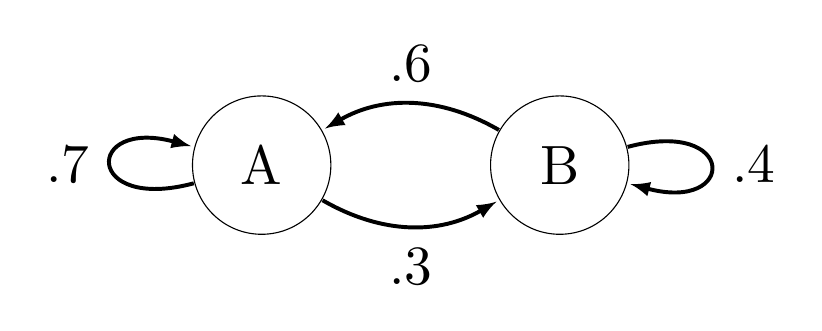
\begin{tikzpicture}[scale=2, every node/.append style={transform shape}]
            % Draw the states
            \node[state]             (A) {A};
            \node[state,right=of A]  (B) {B};
    
            % Connect the states with arrows
            \draw[every loop, line width=.5mm,
            >=latex] 
                (B) edge[bend right, auto=right] node {.6} (A)
                (A) edge[bend right, auto=right] node {.3} (B)
                (B) edge[loop right] node {.4} (B)
                (A) edge[loop left] node {.7} (A);
    \end{tikzpicture}
\end{center}

\noindent
Thus, for a cat starting in State A, after 3 minutes, what is the probability of the cat ending up at State B? 
\end{example}

\begin{solution}
This is where the power of Markov Chains come to use. Using a $n$ x $n$ matrix to depict our probabilities (where $n$ is the number of states), we can utilize matrix exponentiation, or repeated dot products, to find our probabilities. Our starting matrix will look like this:

\[
M=
  \begin{bmatrix}
    .7 & .3 \\
    .6 & .4 
  \end{bmatrix}
\]

\noindent
In the above matrix, we see that each column and row associates with each state. For example, the first column and row relate to State A, where the anything in the first row is out-going from State A and anything in the first column is going into State A. We can see this is true for State B with the second row and column as well.

After using matrix exponentiation to the third power for our 3 minutes (use a calculator if you want), we get a new 3-step transition matrix:

\[
M^{3}=
  \begin{bmatrix}
    .667 & .333 \\
    .666 & .334 
  \end{bmatrix}
\]

\noindent
We can use the same in-going out-going idea using rows and columns with our new matrix as well. To answer our question, we look at the first row for out-going A, and then second column for in-going B. Thus, the probability after 3 minutes that our cat arrives at State B is $.333$.
\end{solution}

\subsection*{Exercises}
Now, here are some problems to try. It's fine to use a calculator for large matrix exponentiations!

\begin{exercise}
    Gain understanding of why we use dot products in Markov Chains. To help, try to draw out a Markov Chain, create a transition matrix, and square it (writing out the calculations by hand).
\end{exercise}

\begin{exercise}
    A group of researchers are analyzing the future possible number of restaurants with vegetarian options. They have determined that every year, originally non-vegetarian restaurants have a $.32$ probability of converting to vegetarian options. Additionally, vegetarian restaurants have $.68$ probability of staying vegetarian every year. In the region, how many restaurants will convert from non-vegetarian to vegetarian on the 5th year, knowing that there are currently $210$ vegetarian restaurants and $320$ non-vegetarian restaurants? 
\end{exercise}

\begin{exercise}
    Stephen is on vacation. Apart from staying in his hotel, he has two other places to spend his time at (for the whole day): the park and the art museum. If he was in his hotel the previous day, he has $.30$ probability of going to the museum and $.42$ probability of going to the park. If Stephen was in the museum the previous day, he has $.60$ probability of spending his time in his hotel and $.21$ probability of going to the park. Last, if we was in the park the previous day, he has $.42$ probability of going to his hotel and $.53$ of going to the park the next day as well. Assuming that he spends his first day at the hotel, what is the probability that he will be at the museum in $4$ days?
\end{exercise}

\end{document}
